\section{Mapping Between SBOL 1, SBOL 2, and SBOL3}
\label{sec:mapping}

In broad strokes, the SBOL 1 standard focused on conveying physical, structural information, whereas SBOL 2 expanded the scope to include functional aspects as well.  
The physical information about a designed genetic construct includes the order of its constituents and their descriptions. 
Specifying the exact locations of these constituents and their sequences allows genetic constructs to be defined unambiguously and reused in other designs. 
SBOL 2 extended SBOL 1 in several ways: it extends physical descriptions to include entities beyond DNA sequences, and it added support for functional descriptions of designs.  
SBOL 3 refined the data model to simplify the representation of common use cases.

\subsection{Mapping between SBOL 1 and SBOL 2}

\ref{SBOL1TO2} depicts the mapping of SBOL 1.1 classes to SBOL 2.x classes, indicating corresponding classes/properties by color.
The SBOL 2.x \sbol{Model} and \sbol{CompenentDefinition} classes have no SBOL 1.1 equivalent, and thus are not shown.
In particular:
\begin{itemize}
\item SBOL 1.1 \external{Collection} objects containing \external{DnaComponent} objects map to SBOL 2.x \sbol{Collection} objects that contain \sbol{CompenentDefinition} objects with DNA \sbolmult{types:CD}{types} properties.
\item SBOL 1.1 \external{DnaComponent} objects maps to SBOL 2.x \sbol{CompenentDefinition} objects with DNA \sbolmult{types:CD}{types} properties.
\item SBOL 1.1 \external{DnaSequence} objects maps to an SBOL 2.x \sbol{Sequence} objects with \external{IUPAC DNA} \sbol{encoding} properties.
\item SBOL 1.1 \external{SequenceAnnotation} objects with \external{bioStart} and \external{bioEnd} properties map to SBOL 2.x\\
\sbol{SequenceAnnotation} objects that contain \sbol{Range} objects.
\item SBOL 1.1 \external{SequenceAnnotation} objects that lack \external{bioStart} and \external{bioEnd} properties map to an SBOL 2.x \sbol{SequenceFeature} objects that contain \sbol{GenericLocation} objects.
\item Each SBOL 1.1 \external{SequenceAnnotation} also maps to an SBOL 2.x \sbol{Component}, which represents the instantiation or usage of the appropriate \sbol{CompenentDefinition}.
\item Each SBOL 1.1 \external{precedes} property maps to an SBOL 2.x \sbol{SequenceConstraint} that specifies a precedes \sbol{restriction} property.
\end{itemize}

\begin{figure*}[h]
\begin{center}
  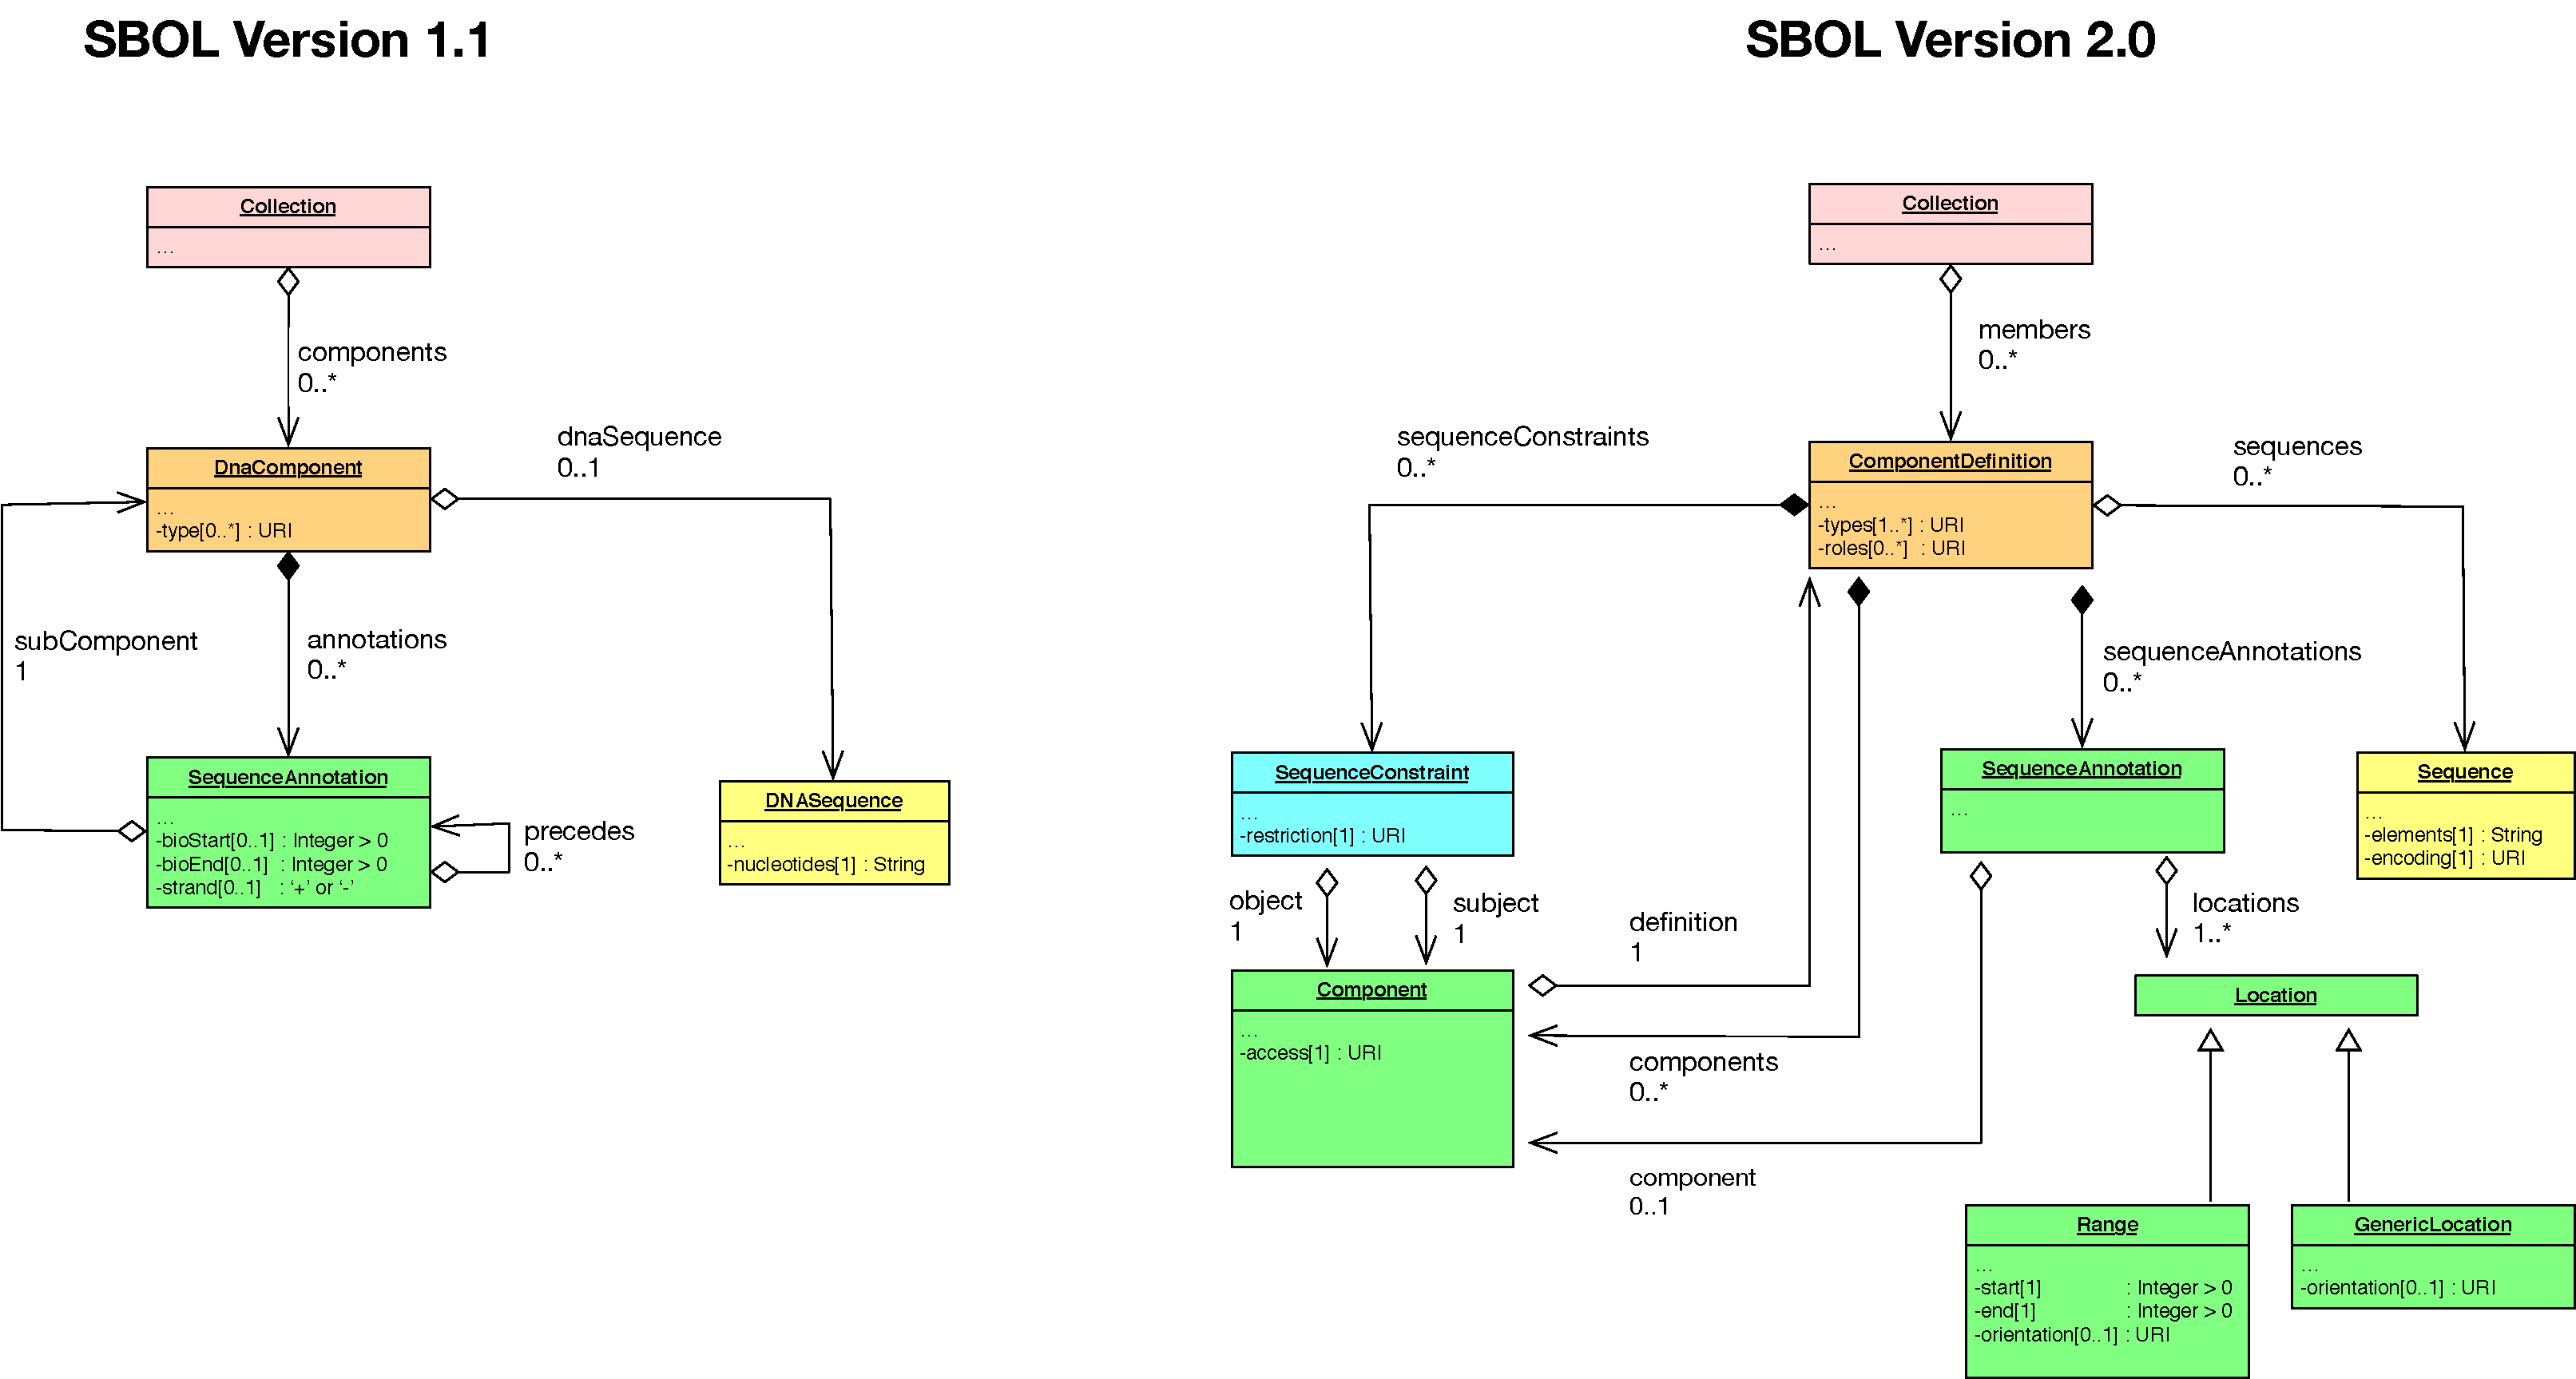
\includegraphics[width=\textwidth]{images/sbol_v1_to_v2}
\end{center}
\caption{\label{SBOL1TO2}The mapping from the SBOL 1.1 data model to the SBOL 2.x  data model, indicating corresponding classes/properties by color.}
\end{figure*}

\subsection{Mapping between SBOL 2 and SBOL 3}

\ref{SBOL1TO2} depicts the mapping of SBOL 2.3 classes to SBOL 3.x classes, indicating corresponding classes/properties by color.
SBOL 3 does not define any new features but streamlines the SBOL 2.3 Data Model.
The highlights are:
\begin{itemize}
	
	\item SBOL 2.3 \external{ComponentDefinition} and \external{ModuleDefinition} objects are merged and map to SBOL 3.x \sbol{Component} objects that contains properties and references from both SBOL 2.3 objects.
	
	\item SBOL 2.3 \external{ComponentInstance} and \external{SequenceAnnotation} objects are unified and maps to SBOL 3.x \sbol{Feature} objects.
	
	\begin{itemize}
		
		\item The derived class from SBOL 2.3 \external{Component} maps to SBOL 3.x \external{SubComponent}
		\item The class from SBOL 2.3 \external{SequenceAnnotation} maps to the SBOL3.x derived class \external{SequenceFeature}.
	\end{itemize}
	
	\item Due to the SBOL 2.3 \external{ModuleDefinition} being unified into SBOL3.x \external{Component} object the functionality to describe directional information is stored in the SBOL 3.x \external{Interface} object that is a property of the SBOL 3.x {Component} object.
	
\end{itemize}

\begin{table}[]
	\begin{tabular}{|l|l|l|}
		\hline
		SBOL 2 Name & SBOL 3 Name & Description \\ 
		\hline
		
		Identified & Identified & \begin{tabular}[c]{@{}l@{}}Removal of Version.\\ 
			Addition of the OM Measure property.\end{tabular} \\
		\hline
		
		TopLevel & TopLevel & Attachments property renamed to has Attachments. \\
		\hline
		
		Sequence & Sequence & Unchanged. \\ 
		\hline
		
		\begin{tabular}[c]{@{}l@{}}ComponentDefinition\\  ModuleDefinition\end{tabular} & Component & \begin{tabular}[c]{@{}l@{}}Merged ComponentDefinition and ModuleDefinition.\\ Renamed Component.\\ From ComponentDefinition Adopted:\\ types,\\ roles,\\ “hasSequences”, \\ “hasFeatures”,\\ “hasConstraints”\\ \\ From ModuleDefinition Adopted:\\ “hasInteraction”,\\ “hasInterface”,\\ “hasModel”\end{tabular} \\
		\hline
		
		ComponentInstance & Feature & \begin{tabular}[c]{@{}l@{}}Renamed to Feature.\\ Component derived class renamed to SubComponent.\\ Addition of ComponentReference, LocalSubComponent, \\ ExternallyDefined and SequenceFeature derived classes.\end{tabular} \\
		\hline
		
		MapsTo & \begin{tabular}[c]{@{}l@{}}Interface, \\ ComponentReference.\end{tabular} & \begin{tabular}[c]{@{}l@{}}Functionality implicitly moved to two new classes.\\ Interface handles directional data.\\ ComponentReference handles ……\end{tabular} \\
		\hline
		
		SequenceAnnotation & SequenceFeature & \begin{tabular}[c]{@{}l@{}}Maps to derived class of Feature that is specially for \\ Annotation on Sequence.\end{tabular} \\
		\hline
		
		Location & Location & \begin{tabular}[c]{@{}l@{}}Removed order property.Removed GenericLocation subclass.\\ Added EntireSequence subclass.\end{tabular} \\
		\hline
		
		SequenceConstraint & Constraint & Renamed to Constraint.Expansion of possible values. \\
		Model & Model & Unchanged. \\
		\hline
		
		Module & SubComponent & \begin{tabular}[c]{@{}l@{}}Merged and mapped when ModuleDefinition is merged \\ into Component.\end{tabular} \\
		\hline
		
		FunctionalComponent & SubComponent & Implicit merge when ModuleDefinition and Module are removed. \\
		\hline
		
		Interaction & Interaction & Participations property renamed to hasParticipations. \\
		\hline
		
		Participation & Participation & Unchanged. \\
		\hline
		
		Collection & Collection & Unchanged \\
		\hline
		
		CombinatorialDeriviation & CombinatorialDeriviation & \begin{tabular}[c]{@{}l@{}}Template now points to Component.\\ variableComponent property renamed to hasVariableComponent.\end{tabular} \\
		\hline
		
		VariableComponent & VariableComponent & Unchanged \\
		\hline
		
		Implementation & Implementation & Unchanged. \\
		\hline
		
		Attachment & Attachment & Unchanged. \\
		\hline
		
		ExperimentalData & ExperimentalData & Unchanged. \\
		\hline
		
		Experiment & Experiment & Now a derived class of Collection. \\
		\hline
		
		Annotation & Annotation & Unchanged. \\
		\hline
		
		GenericTopLevel & TopLevel & Removed. \\
		\hline
		
		Collection & Collection & Unchanged. \\
		\hline
		N/a & Namespace & Derived class of Collection.\\

	\end{tabular}
\end{table}
\begin{figure*}[h]
	\begin{subfigure}{.5\textwidth}
		\centering
		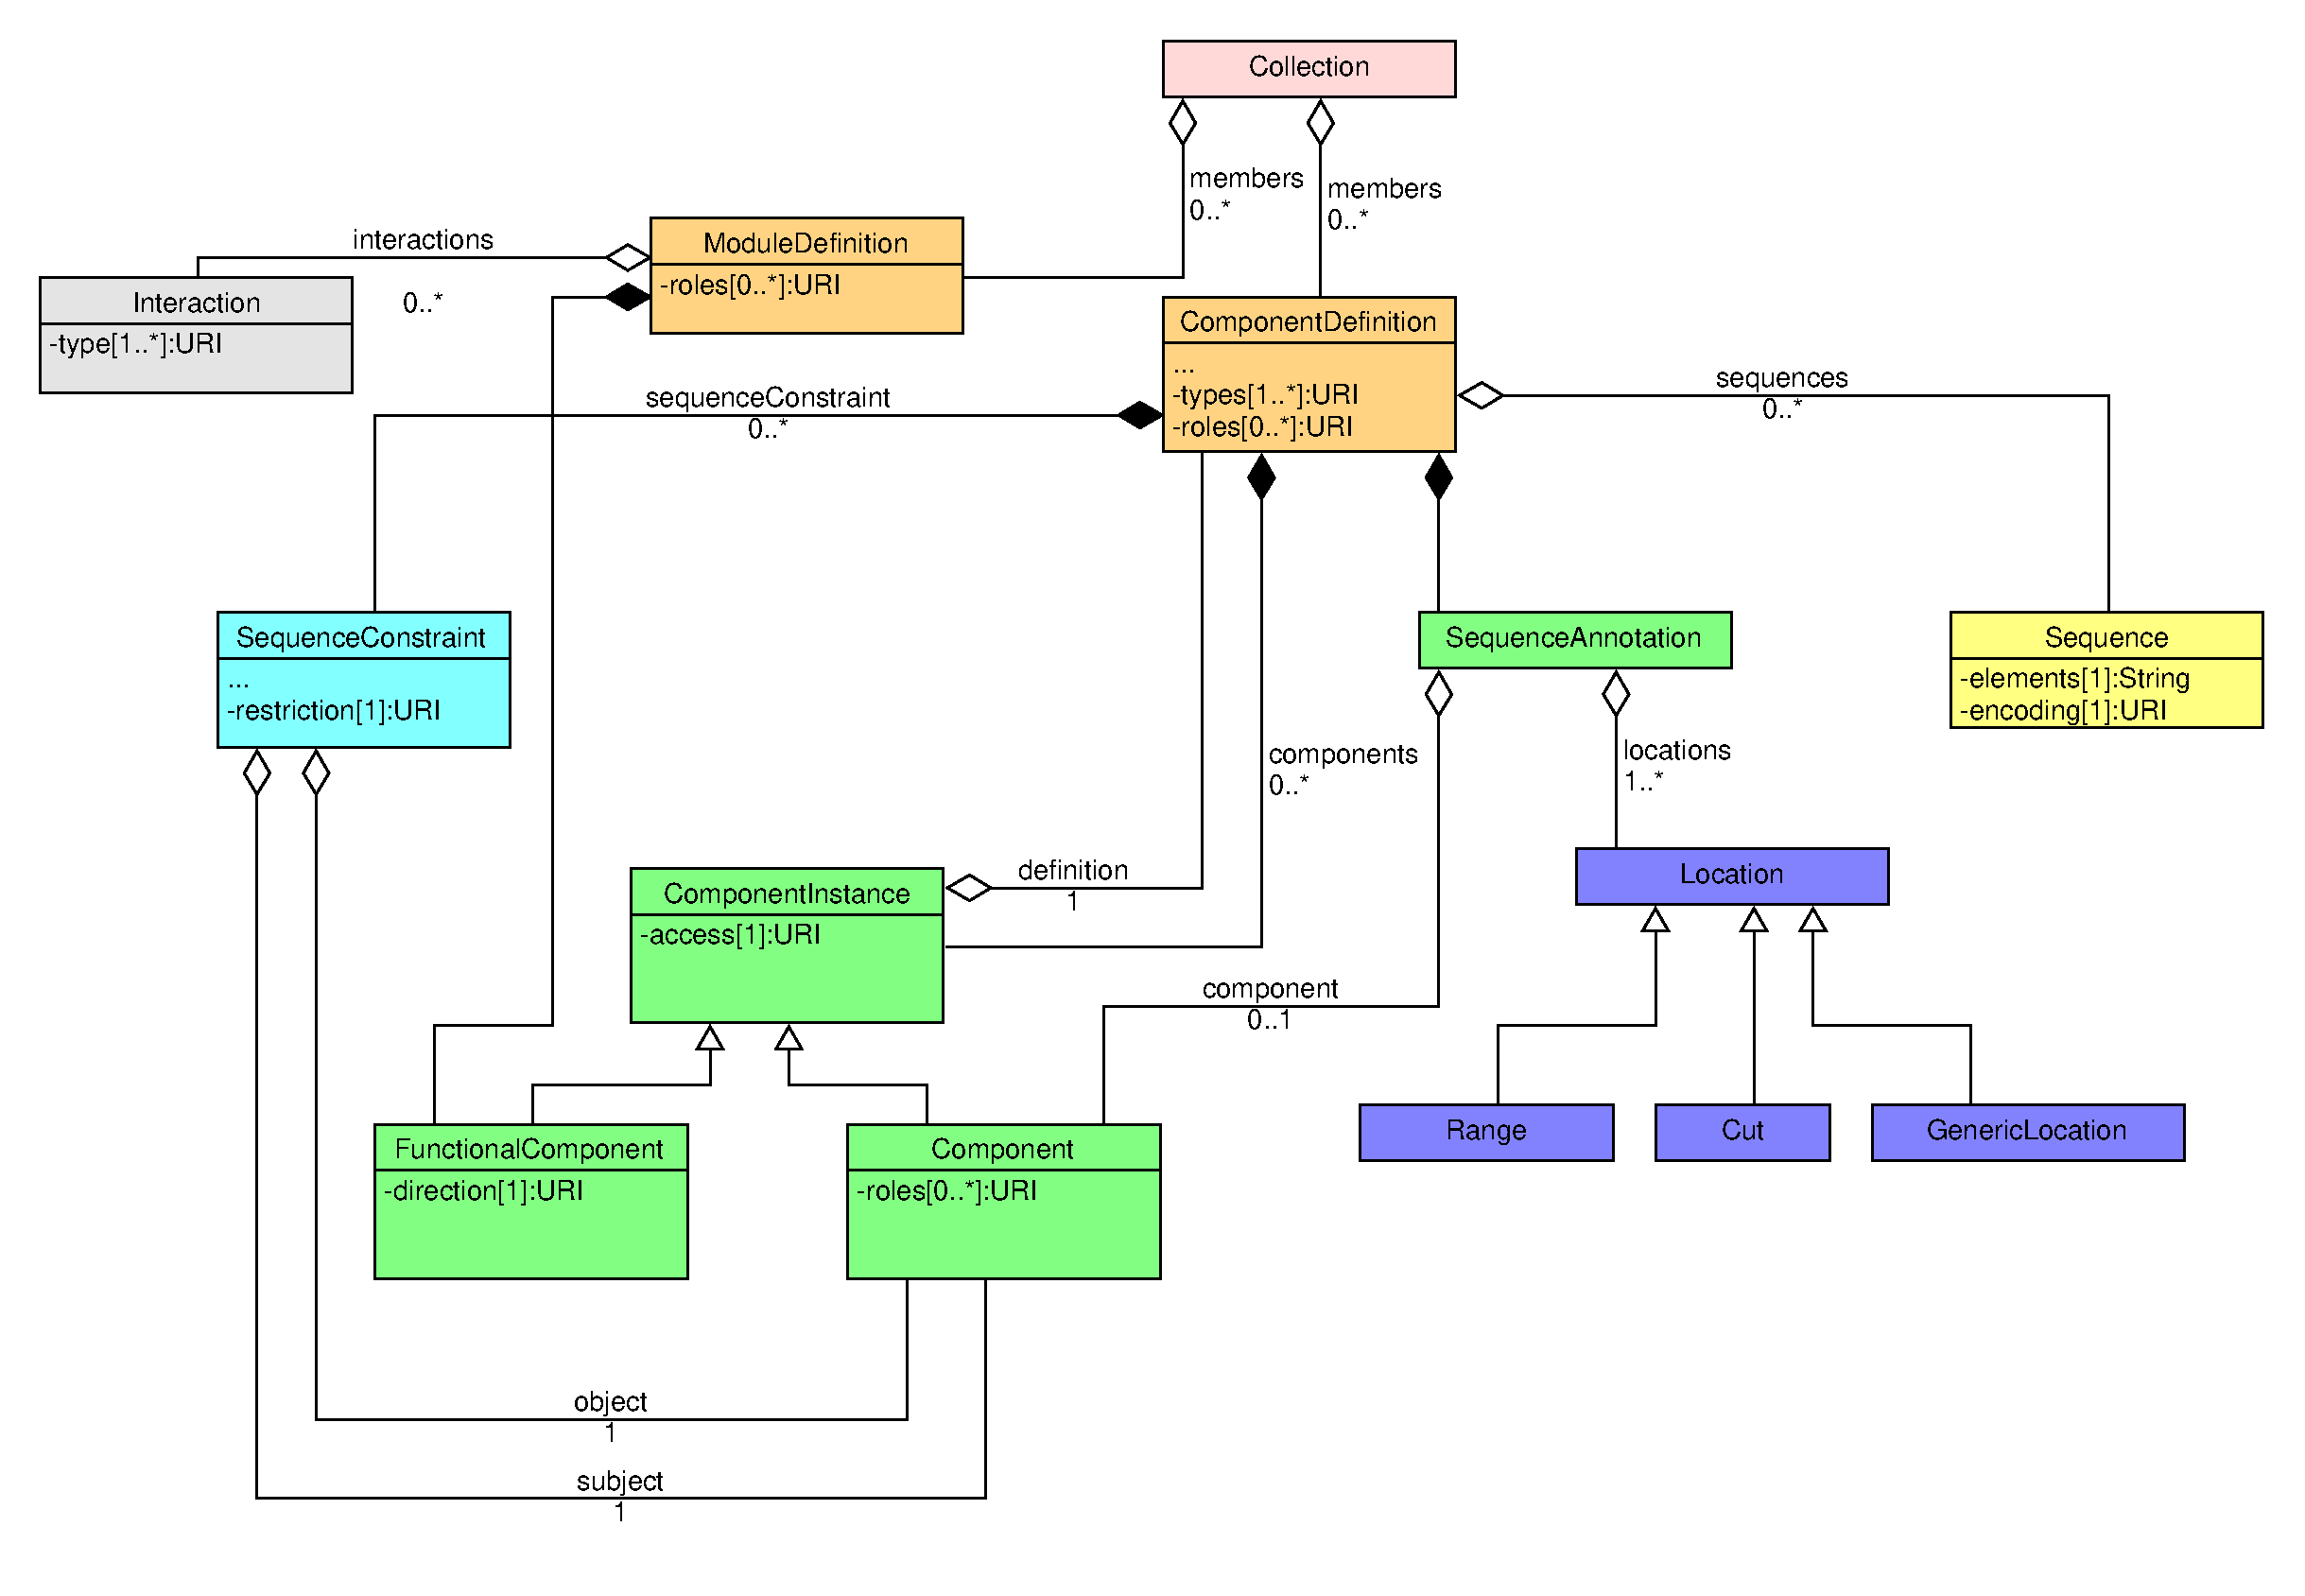
\includegraphics[width=\linewidth]{images/sbol_v2_to_v3_left_subfigure}  
		\caption{SBOL 2.3}
		\label{fig:sub-first}
	\end{subfigure}\begin{subfigure}{.5\textwidth}
		\centering
		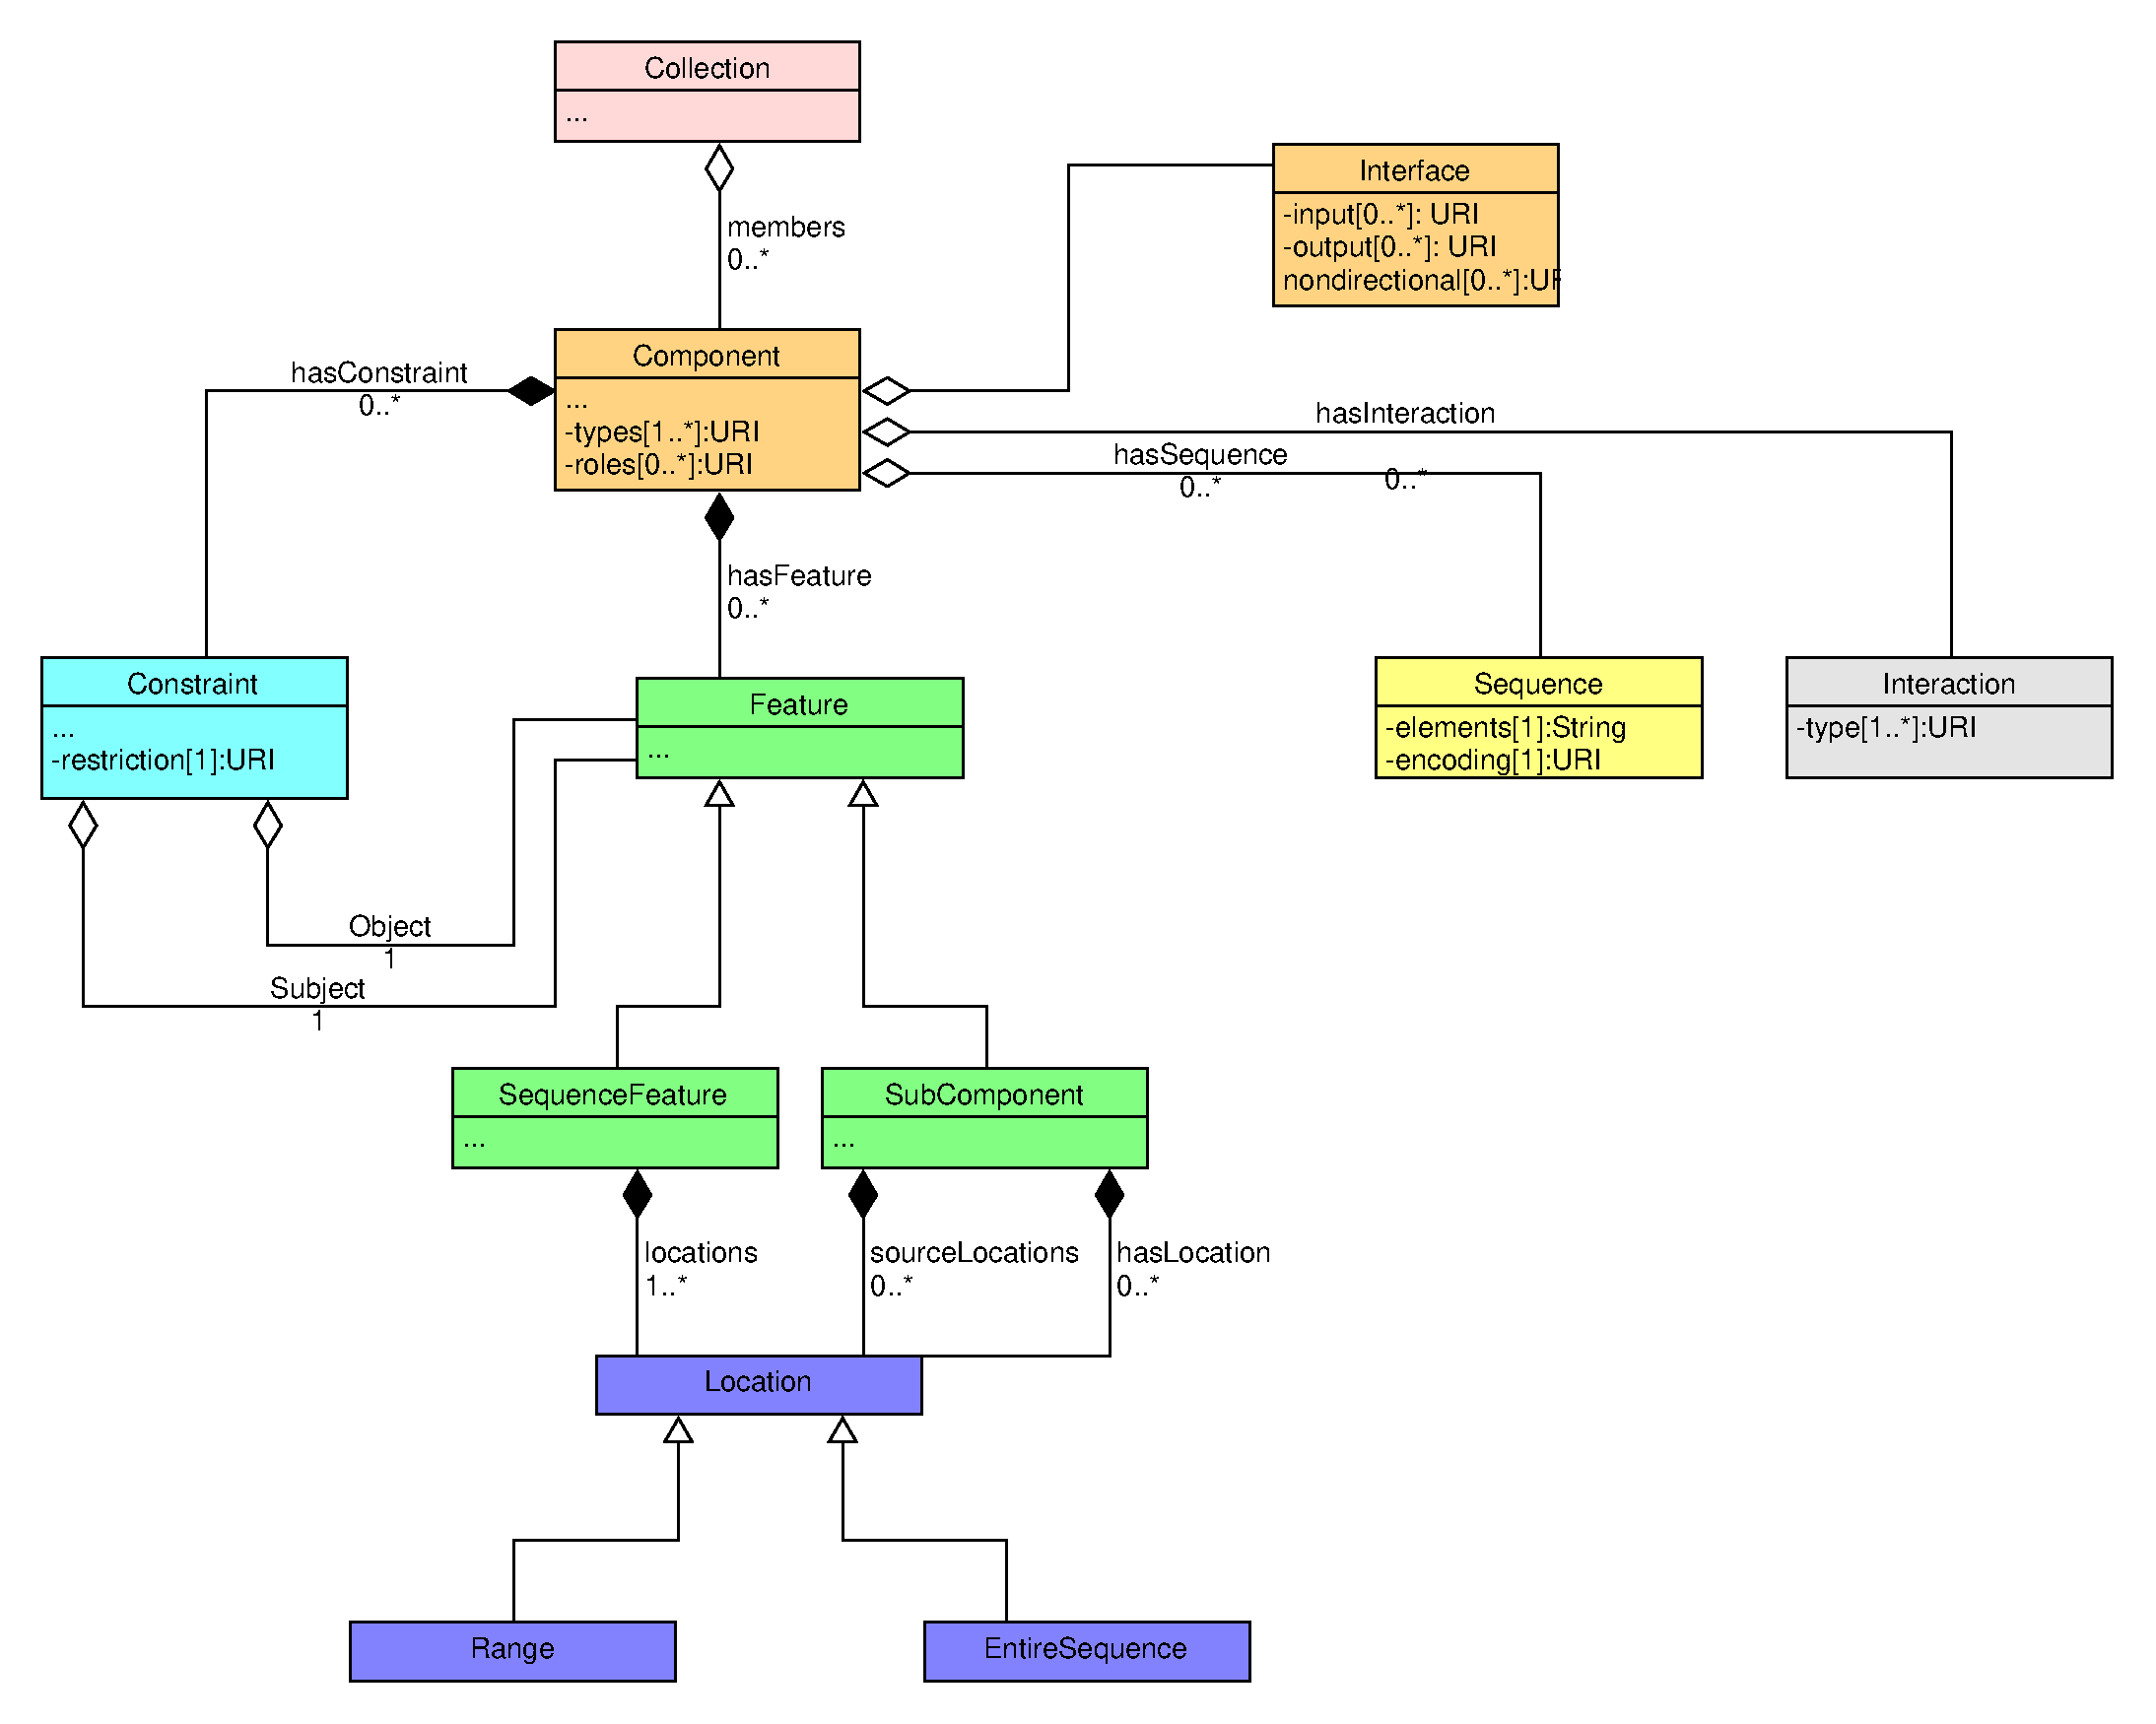
\includegraphics[width=\linewidth]{images/sbol_v2_to_v3_right_subfigure}  
		\caption{SBOL 3.x}
		\label{fig:sub-second}
	\end{subfigure}
	\caption{\label{SBOL2TO3}The mapping from the SBOL 2.3 data model to the SBOL 3.x  data model, indicating corresponding classes/properties by color.}
\end{figure*}